\documentclass[12pt]{article}

\usepackage{fancyhdr}   
\usepackage[utf8]{inputenc} % allow utf-8 input
\usepackage[T1]{fontenc}    % use 8-bit T1 fonts
\usepackage{hyperref}       % hyperlinks
\usepackage{graphicx}    % include graphics
\usepackage{natbib}         
\usepackage{doi}    
\usepackage{listings}
\usepackage{xcolor}
\usepackage{tikz-timing}    % timing diagrams
\usepackage{tikz}
\usepackage{pgfplots}
\usepackage{pgfplotstable}
\usepackage{float}
\usepackage{amsmath}
\usepackage{amssymb}
\usepackage{enumitem}
\setcitestyle{aysep={,}}

% Header information
\newcommand{\Group}{Group Uno}
\newcommand{\Mike}{Mike Orduna}
\newcommand{\Noah}{Noah Murphy}
\newcommand{\Alex}{Alex Livingston}
\newcommand{\Class}{CS 3339: Computer Architecture}
\newcommand{\ReportPart}{Part Three}
\newcommand{\School}{Ingram School of Engineering}

\title{Project Report: \ReportPart}
\author{
    \textbf{\Class} \\
    \\
    \textbf{\Group:} 
    \\
    \Mike\\
    \Noah\\
    \Alex\\
    \\
    \\
    \School
}
\date{\today}

\definecolor{codegreen}{rgb}{0,0.6,0}
\definecolor{codegray}{rgb}{0.5,0.5,0.5}
\definecolor{codepurple}{rgb}{0.58,0,0.82}
\definecolor{backcolour}{rgb}{0.95,0.95,0.92}

\lstdefinestyle{mystyle}{
    backgroundcolor=\color{backcolour},   
    commentstyle=\color{codegreen},
    keywordstyle=\color{magenta},
    numberstyle=\tiny\color{codegray},
    stringstyle=\color{codepurple},
    basicstyle=\ttfamily\footnotesize,
    breakatwhitespace=false,         
    breaklines=true,                 
    captionpos=b,                    
    keepspaces=true,                 
    numbers=left,                    
    numbersep=5pt,                  
    showspaces=false,                
    showstringspaces=false,
    showtabs=false,                  
    tabsize=2
}

\lstset{style=mystyle}
\hypersetup{hidelinks}  % remove colored boxes around links
\usetikzlibrary{automata, positioning}  % automata library for FSMs

\begin{document}
\maketitle
\newpage

\tableofcontents
\thispagestyle{empty}
\pagestyle{fancy}

\newpage
\setcounter{page}{1}

\section{Abstract}

\section{Background}
This report is the third part of a project that aims to develop an ALU using Verilog. The ALU could not be as functional as it is currently without
the previous implementations of the ALU's most basic modules. Throughout the course of the project, design decisions were made to ensure that the ALU
remained modular and easy to understand. That being said, the ALU was chosen to follow a \textit{hierarchical design} approach, where the ALU is built
from smaller modules.

Development of the ALU began with implementing its most basic functions: \textit{Logic Gates}. Implementation starts with making modules for these basic
gates, which are then used to develop more complex modules down the line. In the first report discussed, the primary focus was ensuring that these logic
gates received the fed inputs correctly and produced the expected outputs. Furthermore, the development of a basic arithmetic shifter was implemented in
conjunction with the logic gates, as required by the project's first step. These files can be viewed under the \textbf{src} directory, and more specifically
refer to the files \textit{bit\_gates.v}, \textit{nbit\_gates.v}, and \textit{arithmetic\_operations.v}. Other modules made in this section include the
\textit{checks.v} and the \textit{mxnbit\_gates.v} files which offer additional functionality outside of the specifications of the project.

Afterwards, the development of the core functions of the ALU were implemented. This included the basic mathematical operations of an ALU: addition,
subtraction, multiplication, and division. Following the guidelines developed during the planning of the project, this section of the ALU is built on
many of the logic gates previously developed and make use of Verilog's \textit{generate} statements to instantiate the appropriate modules for each
operation. The modules refer to the files \textit{arithmetic\_operations.v} and the later added \textit{combinational\_alu.v} files. In earlier versions
of this part of the project, the operations for the ALU went through many different iterations and were all shared in the same file. However, after 
much evaluation, a separation of concerns was established and enforced between the two core functions, leading to the split of the files.

While the initial project phases emphasized the development of the ALU's core functions, the later phases of the project focus on the refinement of
the ALU's modules. Moreover, the later phases of the project focus on the introduction of a controller to the ALU, allowing for it to perform its
calculations more realistically and sequentially.

\section{Introduction}
An ALU's effectiveness is not only determined by its ability to perform arithmetic operations, but also by its ability to manage the flow of these
operations over a period of time. In earlier stages of the project, the ALU's primary focus was functionality and correctness of the operations. However,
moving from the core functions of the ALU to the controller, the focus shifts to the overall control the ALU has over its operations.

The introduction of control logic to the ALU transforms it from a purely combinational circuit into one that is sequential. This means that the ALU
would process instructions fed into it over multiple clock cycles. This change in fundamental processing allows for an ALU to synchronize its operations,
managing its time and resources more effectively. In this report, a focus on the developmental process of the ALU controller is discussed, including the
methods used to implement the controller, the challenges faced during development, and the solutions that were developed to overcome these challenges.

\section{Controller Design}
The controller is the most important aspect of an ALU, as it is responsible for directing the flow of data and operations within the ALU. A controller
is a sequential circuit that takes in inputs and produces outputs based on the current state of the system. 

\subsection{Controller Inputs and Outputs}
To design the controller, defining its inputs and outputs is essential. There are two types of inputs to a controller: the timing inputs and the ALU inputs.
The timing inputs are the signals that are used to control the timing of the controller's operations and include the following:
\begin{itemize}
    \item \textbf{Clock}: The clock signal is used to synchronize the operations of the ALU. It is a periodic signal that is used to trigger the controller's state transitions.
    \item \textbf{Reset}: The reset signal is used to initialize the controller to a known state. It is an active high signal that resets the controller's state.
    \item \textbf{Start}: The start signal is used to indicate that the ALU should begin processing an operation. It is an active high signal that triggers the controller to start its operation.
\end{itemize}

The ALU inputs are the signals that are used to determine and perform the operation to be performed by the ALU. These inputs include the following:
\begin{itemize}
    \item \textbf{Opcode}: The opcode is a binary representation of the operation to be performed by the ALU. It is a multi-bit signal that is used to select the operation to be performed.
    \item \textbf{Input 1}: The first input to the ALU. It is a multi-bit signal that is used as the first operand for the operation.
    \item \textbf{Input 2}: The second input to the ALU. It is a multi-bit signal that is used as the second operand for the operation.
\end{itemize}

The primary output is split into three outputs: a high, a low, and a flag. This is to accommodate the different methods of outputting from the individual ALU operations.
The outputs are as follows:
\begin{itemize}
    \item \textbf{High Output}: The high output is a multi-bit signal that is used to indicate the high portion of outputs. Primarily used in multiplication, division, or shift operations.
    \item \textbf{Low Output}: The low output is a multi-bit signal that is used to indicate the low portion of outputs. This is used to represent the remaining operations such as addition or subtraction
        as well as the low portion of multiplication and division or the shift result.
    \item \textbf{Flag}: The flag is a single bit signal that is used to represent carry, borrow, or comparison flags.
\end{itemize}

The controller has an output to mark its completion labeled as \textit{done}. This is a single bit signal that is used to indicate that the ALU has completed its operation and is ready to output
the result.

\subsection{Separation of Concerns}
In order to facilitate the development of the controller, a separation was established between the main ALU controller and the sub-controllers. 
\begin{itemize}
    \item \textbf{Sequential Controller}: Acts as the main controller for the ALU. It is responsible for managing the overall flow of the ALU operations and directing the sub-controllers to perform their respective operations.
    \item \textbf{Sub-Controllers}: These are the individual controllers that are responsible for performing the specific operations of the ALU. Each sub-controller is responsible for a specific operation, such as addition, 
        subtraction, multiplication, or division.
\end{itemize}

\subsection{When to Use a Controller?}
In the design of the ALU's controller, it was important to ask when to develop a controller for a specific module. Not every operation in an ALU requires a controller, as in some cases operations
are done in one clock cycle as opposed to a span of cycles. Since the combinational logic was split in its core operations, it was deduced that those operations, operations with a \textit{core} unit 
attached to them would need to be controlled by some central controller. This meant that modules such as the shifter, the comparator, and the logic gates would not need a controller, while remaining
modules would.

Furthermore, since the ALU controller was split into two function, it would not be ideal for both the ALU controller and the sub-controllers to be sequential. Had both controllers included sequential logic, 
the interaction between their clock cycles would create more complicated timing mismatches, which in turn would require more complex logic to manage. So it was declared that the ALU controller would solely 
be combinational, while still housing the timing inputs to feed into the sub-controllers; those of which did function on the timing inputs. This design decision allowed for the separation of concerns between 
the different controllers developed for the ALU and allowed for a more modular design.

\section{Testbench Development}
To test the functionality of the controllers developed, two generic tests were designed and made, similarly to how they were discussed in the previous report, \textit{Part Two}. These tests iterated through
every potential input combination possible for the ALU. More specifically, it incremented the 3 primary inputs in the ALU: the opcode, input 1, and input 2. 

\subsection{Testbench Design}
The tests also needed to include some method of tracking the clock and reset signals so that the ALU could be properly initialized and run for each change in input. In order to properly capture the correct 
change in output for each change in input, posedge detections were added into the generic tests. These posedges are used to tell the controller to update its state and output registers. However, applying a
posedge requires a careful consideration for where they are placed in the generic tests to avoid saturating the system with too many posedges and that it updates its outputs accordingly. The general rules
to follow when adding posedges are:
\begin{itemize}
    \item \textbf{Posedge Between Input Change}: This is to ensure that the controller updates its state and output registers before the next input change.
    \item \textbf{Posedge Between Control Transitions}: This is to ensure that the controller updates its state and output registers before the next control transition.
    \item \textbf{Posedge After Setting Done Signals}: This is to ensure that the controller updates its state and output registers after the done signal is set.
\end{itemize}

\subsection{Testbench Implementation}
The testbench was implemented in a separate file, \textit{testbench\_sequential.v}. This file tested two both the ALU controller and the sub-controllers.

\subsubsection{Sub-Controller Testing}
Testing was first done on the sub-controllers, as they
relied on their \textit{core} units. Developing these controllers first allowed for a more modular design to be implemented across the different sub-controllers, as we would be testing for similar functionality
across the different modules. The testbench developed for the sub-controllers is shown below:
\begin{lstlisting}[language=Verilog]
    `define GENERIC_CONTROL( REG1, REG2, CLK, RESET, START, DONE ) \
    begin \
        RESET = 1'b0; START = 1'b0; \
        REG1 = { WIDTH{ 1'b0 } }; \
        repeat( BIT_STATE ) begin \
            REG2 = { WIDTH{ 1'b0 } }; \
            repeat( BIT_STATE ) begin \
                RESET = 1'b1; @( posedge CLK ); \
                RESET = 1'b0; @( posedge CLK ); \
                @( posedge CLK ); \
                START = 1'b1; @( posedge CLK ); \
                START = 1'b0; \
                wait( DONE ); \
                @( posedge CLK ); @( posedge CLK ); \
                REG2 = REG2 + 1; @( posedge CLK ); \
            end \
            REG1 = REG1 + 1; @( posedge CLK ); \
        end \
        REG1 = {WIDTH{1'b0}}; \
        REG2 = {WIDTH{1'b0}}; \
    end
\end{lstlisting}

The test was implemented using a macro to allow for a generic test to be used with any of the different controllers. The macro takes in the following parameters:
\begin{itemize}
    \item \textbf{REG1}: The first register to be tested. This is the register that will be used to store the first input to the ALU.
    \item \textbf{REG2}: The second register to be tested. This is the register that will be used to store the second input to the ALU.
    \item \textbf{CLK}: The clock signal for the ALU. This is the signal that will be used to synchronize the operations of the ALU.
    \item \textbf{RESET}: The reset signal for the ALU. This is the signal that will be used to initialize the ALU to a known state.
    \item \textbf{START}: The start signal for the ALU. This is the signal that will be used to indicate that the ALU should begin processing an operation.
    \item \textbf{DONE}: The done signal for the ALU. This is the signal that will be used to indicate that the ALU has completed its operation and is ready to output the result.
\end{itemize}

Each timing input is carefully placed to ensure that the system is able to record and process the inputs correctly. One mismatch in the timing of the inputs could
lead to a loss of information, where old data is saved or data that does not exist yet is used. This is why the timing of the inputs is so important in the design of
the controller. 

\subsubsection{Clock Signal Implementation}
Notice that the clock signal is not included in the macro directly; there is no CLK that is incremented in the macro. Rather, the clock is initialzied outside of the macro, 
in the testbench. There are a few standard methods for which to increment a clock depending on the application. For the purpose of this testbench, a simple implementation
was used to increment the clock:
\begin{lstlisting}[language=Verilog]
    initial begin
        clk = 1'b0;
        # Inverts the clock every 5 time units
        forever #5 clk = ~clk;
    end
\end{lstlisting}

This implementation increments the clock signal every 5 time units, which is set to 1ns for the purpose of this testbench. This means that the clock signal will toggle every 5ns
forever, until the simulation is stopped. This is a simple implementation of a clock signal that is used to synchronize the operations of the ALU.

\subsubsection{ALU Controller Testing}
Testing for the ALU controller was done in a similar fashion to the sub-controllers, with the only difference being an extra input to the macro: the opcode. The opcode is placed
at the beginning of the macro, as it is the first input to be changed. The opcode is then incremented in a loop after the remaining test is concluded. For every opcode, the generic
test listed above is conducted.

\subsection{Testbench Timing Diagrams}
At the lowest level of the testbench, the clock, reset, and start signals make up a single input change. This change is represented by the timing diagram shown below.
\begin{figure}[H]
    \centering
    \begin{tikztimingtable}[timing/slope=0, xscale=1.2]
    CLK & 12{LH} \\
    RST & H 22L 1H \\
    START & 5L 2H 17L \\
    DONE & 18L 2H 4L \\
    \end{tikztimingtable}
    \caption{Timing diagram showing one ALU controller activation cycle with a reset phase, input start pulse, and synchronization to the system clock.}
\end{figure}

The diagram illustrates the signal timing associated with a single change in input. The \texttt{CLK} signal remains periodic with a constant cycle length. This is the
result of the code mentioned in the \textit{Clock Signal Implementation} section. The \texttt{RST} (reset) signal is asserted at the beginning to initialize the system and then
deasserted after the first rising edge. It remains low for most of the operation and is reasserted at the end to reset the state for the next operation. The \texttt{START} signal 
is asserted for two clock cycles after reset is deasserted, signaling the controller to begin executing the operation based on current inputs. The \texttt{DONE} signal is asserted 
for two clock cycles once the operation is complete, indicating the result is available and the controller is ready for the next input.

All control signals (\texttt{RST}, \texttt{START}, and \texttt{DONE}) are held high for \textit{two full clock cycles} rather than one to ensure the controller registers each transition
reliably. This design choice prevents race conditions and ensures that state changes are properly latched. The effect of this timing strategy will become more evident in later sections
when the behavior of the sub-controllers is analyzed.

\subsection{Testbench Module Instantiations}
In order to use the macro in the testbench, the modules to be tested need to be instantiated in the testbench. This is done by creating instances of the modules that are to be tested
and passed into the macro. One example of this is shown below, where the \textit{Addition\_Control} module is instantiated in the testbench:
\begin{lstlisting}[language=Verilog]
    /*
     * Addition_Control module instantiation
     */
    reg [ WIDTH-1:0 ] add_in1, add_in2;
    wire [ WIDTH-1:0 ] add_out;
    wire add_done, final_carry;

    Addition_Control #( .WIDTH( WIDTH ) ) add_control_instance (
        .clk( clk ),
        .reset( reset ),
        .start( start ),
        .in1( add_in1 ),
        .in2( add_in2 ),
        .out( add_out ),
        .final_carry( final_carry ),
        .done( add_done )
    );

    // Latch the output signals for clearer waveform
    reg [WIDTH-1:0] add_latched;
    reg carry_latched;
    always @(posedge clk) begin
        if( add_done ) begin
            add_latched <= add_out;
            carry_latched <= final_carry;
        end
    end
\end{lstlisting}

Every module tested is instantiated the same way, with differences being the naming of input variables and module names. 

\subsubsection{Latch Implementation}
It is important to note the use of a \textit{latch} for the output signals. The outputs from each module vary or oscillate with the periodic clock due to the internal combinational 
circuitry, which can produce intermediate values between clock edges. To avoid an oscillating output, the output signal can be latched using a flip-flop register. The latching is 
done using a simple always block that captures the output of the module when the \texttt{DONE} signal is asserted. This ensures a stable output value is captured until the next 
operation is completed.

\section{ALU Controller}
The ALU controller is the top-level controller for the ALU, as it designates the flow of data and operations within the ALU. The inputs and outputs of the ALU controller are discussed
in the \textit{Controller Inputs and Outputs} section.

\subsection{ALU Operations}
The ALU controller directs the flow of data using a finite state machine, which manages operation selection and output coordination. Although FSMs are typically sequential, the ALU FSM
was designed to act as a purely combinational block to mitigate timing mismatches between the controller and sub-controllers. In order to maintain the modularity and hierarchical design, 
the ALU instantiates the sub-controllers before entering its FSM. Because of this, every operation in the ALU is computed per input. However, once the FSM is entered, only the specified 
operation is transferred and outputted by the ALU controller module.

\subsubsection{ALU Controller States}
The ALU controller is designed to handle the following operations with the assigned opcodes:
\begin{figure}[H]
    \centering
    \begin{tabular}{|c|c|c|}
        \hline
        \textbf{Operation} & \textbf{Opcode}    \\
        \hline
        \texttt{Addition} & 0000 \\
        \texttt{Subtraction} & 0001 \\
        \texttt{Multiplication} & 0010 \\
        \texttt{Division} & 0011 \\
        \texttt{Logical Shift} & 0100 \\
        \texttt{Arithmetic Shift} & 0101 \\
        \texttt{Greater Than} & 0110 \\
        \texttt{Less Than} & 0111 \\
        \texttt{Equal To} & 1000 \\
        \texttt{Bitwise AND} & 1001 \\
        \texttt{Bitwise OR} & 1010 \\
        \texttt{Bitwise XOR} & 1011 \\
        \texttt{Bitwise NOT} & 1100 \\
        \hline
    \end{tabular}
    \caption{ALU Opcode Table}
\end{figure}

One thing to note about the ALU operations is the difference between the logical and arithmetic shifts. \textit{Logical shifts} are used to shift the bits of a number to the left or
right, filling the empty bits with zeros. This is useful for unsigned numbers, where the sign of the number does not matter. \textit{Arithmetic shifts}, on the other hand, are used to shift
the bits of a signed number to the left or right, filling the empty bits with the sign bit. This is useful for signed numbers, where the sign of the number matters. Both of these shifts carry
their own control signals within them and are used to determine the direction of the shift, the amount of bits to shift, and the fill bit to use. 

\subsubsection{Sub-Controller Instantiations}
The ALU controller instantiates the sub-controllers for each operation to be performed. This is a feature of the ALU controller that allows for the modularity of the design to be maintained
more easily. This also allows for the ALU to pass down the responsibility of the operations to the sub-controllers, rather than having all the logic in the ALU controller. However, this does
impact the performance of the ALU, as the ALU controller must wait for the sub-controllers to complete their operations before it can proceed, even when the operation is not needed.

Each sub-controller is instantiated such like:
\begin{lstlisting}[language=Verilog]
    // Addition Controller
    wire [ WIDTH-1:0 ] add_out;
    wire add_done, final_carry;

    Addition_Control #( .WIDTH( WIDTH ) ) adder_instance (
        .clk( clk ),
        .reset( reset ),
        .start( start ),
        .in1( in1 ),
        .in2( in2 ),
        .out( add_out ),
        .final_carry( final_carry ),
        .done( add_done )
    );
\end{lstlisting}

Most of the sub-controllers are instantiated in a similar fashion, with the differences being the naming conventions and the output signals. The instantiations allow for a modular and cleaner design, 
as the ALU controller becomes a simple wrapper around the sub-controllers. This allows for the ALU controller to be easily modified or extended in the future, as new operations can be added by simply
adding a new sub-controller and updating the ALU controller to include the new operation. This is a key feature of the hierarchical design approach taken in this project.

\subsubsection{ALU Finite State Machine}
The finite state machine for the ALU controller is designed to be purely combinational. It selects and coordinates which of the sub-controllers outputs to use based on the opcode. The FSM for
the ALU was originally designed to be sequential, but due to timing mismatches between the ALU controller and the sub-controllers, it was changed to be purely combinational. This change
allows for easier debugging and readability at the cost of performance. Sequential logic is typically easier to debug and understand than combinational logic, since the flow of the data using
case statements and a clock is easier to follow than a looped combinational circuit. However, this change does not impact the functionality of the ALU, as the ALU controller is still able to
perform its operations correctly. The FSM is shown below:
\begin{lstlisting}[language=Verilog]
    always @(*) begin
        // Initialize the output signals
        out_high = { WIDTH{ 1'b0 } };
        out_low = { WIDTH{ 1'b0 } };
        flag = 1'b0;
        done = 1'b0;

        case( opcode )
            ADD: begin
                out_low = add_out;
                flag = final_carry;
                done = add_done;
            end
            SUB: begin
                out_low = sub_out;
                flag = final_borrow;
                done = sub_done;
            end
            ... and so on
\end{lstlisting}

This pattern continues for all available operations, where the different outputs are assigned based on which operation is selected. Not every output in the ALU controller is assigned due to
either a limited representation of the output or the lack of need for the output. Due to how the operations performed have varying output sizes, the outputs from the ALU remain flexible.

\section{Sub-Controllers}
The sub-controllers are the individual controllers of their respective operation. Of the operations performed by the ALU, there are only four operations that required sub-controllers:
\begin{itemize}
    \item \textbf{Addition}
    \item \textbf{Subtraction}
    \item \textbf{Multiplication}
    \item \textbf{Division}
\end{itemize}

Each of these operations performed their calculations in a series of steps, and originally used loops to perform their operations. However, after some refactoring of the modules, the operations
were changed to accommodate the new design of the ALU. Each sub-controller now incorporates a finite state machine (FSM) with a well-defined state transition process to manage the step-by-step 
execution of its operation. This in turn added additional clarity to the design of the ALU, and furthermore, allowed the operations to be performed in a sequential manner rather than combinational. 
It is important to note that this is in accordance to how real hardware operates, as hardware takes time to produce results.

\subsection{Sub-Controller Operation}
Each sub-controller runs in a sequential manner. The sub-controller is activated by the ALU controller, which then runs through its FSM to perform the operation. The FSM is broken down into
parts that are responsible for the different steps of the operations and all remain relatively similar in design. The general structure of the FSM is as follows:
\begin{itemize}
    \item \textbf{IDLE}: The initial state of the FSM. The FSM waits for the start signal to be asserted before proceeding to the next state.
    \item \textbf{INIT}: The initialization state of the FSM. The FSM initializes the input registers and sets the output registers to zero.
    \item \textbf{STEP}: The main state of the FSM. The FSM performs the operation and updates the output registers.
    \item \textbf{LOAD}: The load state of the FSM. The FSM loads the output registers with the final result.
    \item \textbf{DONE}: The final state of the FSM. The FSM sets the done signal and resets the state to IDLE.
\end{itemize}

The done signal is asserted by sub-controllers to indicate completion of their operation. The ALU controller monitors these flags to determine when to latch the outputs and re-enter the IDLE state.
This handshake ensures synchronization between sequential and combinational logic blocks.

Below are two state diagrams describing how their respective controllers flow during runtime:

\begin{figure}[H]
    \centering
    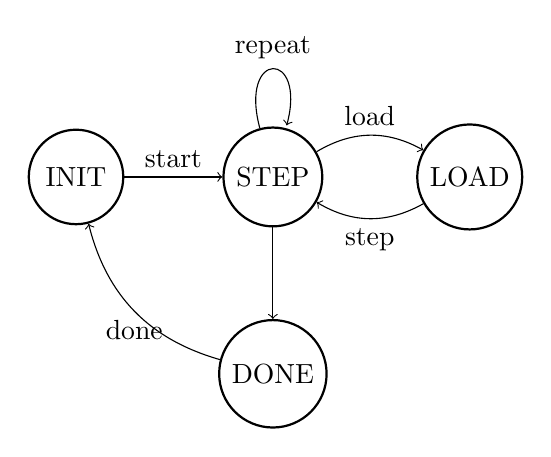
\begin{tikzpicture}[->, node distance=2.5cm, every state/.style={thick, minimum size=1.2cm}]
        \node[state] (A) {INIT};
        \node[state] (B) [right of=A] {STEP};
        \node[state] (C) [right of=B] {LOAD};
        \node[state] (D) [below of=B] {DONE};

        \path
            (A) edge node[above] {start} (B)
            (B) edge[loop above] node {repeat} (B)
            (B) edge[bend left] node[above] {load} (C)
            (C) edge[bend left] node[below] {step} (B)
            (B) edge node {} (D)
            (D) edge[bend left] node[below] {done} (A);
    \end{tikzpicture}
    \caption{State diagram of the Addition and Subtraction Controllers}
    \label{fig:add_sub}
\end{figure}

\begin{figure}[H]
    \centering
    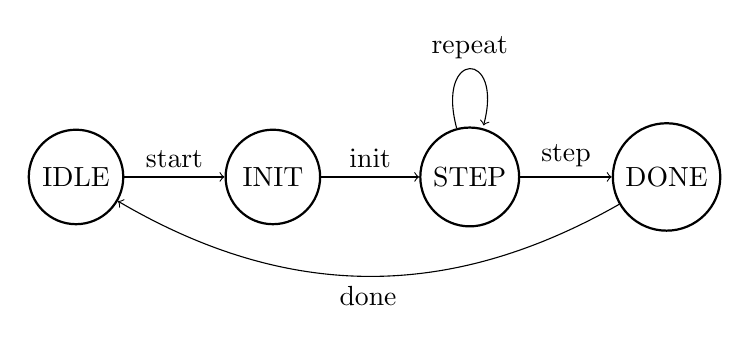
\begin{tikzpicture}[->, node distance=2.5cm, every state/.style={thick, minimum size=1.2cm}]
        \node[state] (A) {IDLE};
        \node[state] (B) [right of=A] {INIT};
        \node[state] (C) [right of=B] {STEP};
        \node[state] (D) [right of=C] {DONE};

        \path
            (A) edge node[above] {start} (B)
            (B) edge node[above] {init} (C)
            (C) edge node[above] {step} (D)
            (C) edge[loop above] node {repeat} (C)
            (D) edge[bend left] node[below] {done} (A);
    \end{tikzpicture}
    \caption{State diagram of the Multiplication and Division Controllers}
    \label{fig:div_mult}
\end{figure}

While most of the states are similar across the different sub-controllers, the \textit{INIT} and \textit{LOAD} states are featured in their own unique manner. The \textit{INIT} state is used to
initialize the input registers in the \textit{addition} and \textit{subtraction} operations while the \textit{LOAD} state is used to load registers in the \textit{multiplication} and \textit{division} 
operations. This is due to the designs of each respective operation and will be discussed in more detail in the following sections. However, the FSM logic for the sub-controllers are all designed
to move through each state as the operation is performed.

Furthermore, every operation receives a section before the FSM case logic is entered that initializes any internal wires and output registers used in the operation. This helps each input to be independant
from one another and avoid any mismatches in the timing of the inputs. This is denoted in the source files as a check against \texttt{RESET} during runtime.

\subsection{Adder Controller}
The Adder controller is the first of the sub-controllers developed and is responsible for performing the addition operation. It is composed of the 2 main parts:
\begin{itemize}
    \item \textbf{Adder Core}: The core unit that performs the addition operation. It is a simple combinational circuit that takes in two bits and produces a sum and a carry bit.
    \item \textbf{Adder Controller}: The controller that manages the flow of the addition operation. It is a sequential circuit that directs the \textit{Adder Core} to perform the
        addition of the inputs over multiple clock cycles.
\end{itemize}

\subsection{Adder Core}
The \textit{adder core} is the combinational circuit refactored from the previous report. It performs its functions on a bit-by-bit basis, where each bit is added together and the carry is
added and passed to the next bit. The difference between the previous implementation and the current implementation is that the logic of the bit-by-bit process is now separated from the
combinational logic it was in before. This allows for it to be used either in a combinational or sequential manner, depending on the needs of the design.

The \textit{adder core} remains the same, as it is composed of two half adders, one for each input and one for the carry bits, and an OR gate to determine the final carry. The
\textit{adder core} is shown below:

\begin{lstlisting}[language=Verilog]
module Addition_Core #( parameter WIDTH = 4 ) (
    input wire in1,
    input wire in2,
    input wire carry_in,
    output wire out,
    output wire carry_out
);
    // Internal wires
    wire temp_out, temp_carry_out, carry_overflow;

    // Add the inputs and store the output
    Half_Adder input_adder_instance (
        .in1( in1 ),
        .in2( in2 ),
        .out( temp_out ),
        .carry_out( temp_carry_out )
    );

    // Add the carry
    Half_Adder carry_adder_instance (
        .in1( temp_out ),
        .in2( carry_in ),
        .out( out ),
        .carry_out( carry_overflow )
    );

    // Determine the final carry
    OR or_instance (
        .in1( temp_carry_out ),
        .in2( carry_overflow ),
        .out( carry_out )
    );
endmodule
\end{lstlisting}

\subsection{Adder Controller FSM}
From the \textit{adder core}, the \textit{adder controller} is built. It uses an FSM to manage the different states the addition operation can be in and uses the \textit{adder core} to perform each
step of the addition of two inputs. The addition FSM first moves into the \texttt{INIT} state, where the input registers are initialized. It then moves into a switching between \texttt{STEP} and
\texttt{LOAD} states, where the addition is performed and then is saved to the output registers and for the next carry bit. The FSM is shown below:
\begin{lstlisting}[language=Verilog]
    case( state )
        INIT: begin // Initialize the addition operation
            done <= 1'b0;
            if( start ) begin
                step_counter <= 0;
                current_in1 <= in1[ 0 ];
                current_in2 <= in2[ 0 ];
                carry_in <= 1'b0;
                state <= LOAD;
            end
        end
        STEP: begin // Perform the addition operation
            if( step_counter < WIDTH ) begin
                current_in1 <= in1[ step_counter ];
                current_in2 <= in2[ step_counter ];
                carry_in <= carry_out;
                state <= LOAD;
            end else begin
                out <= final_out;
                final_carry <= carry_out;
                state <= DONE;
            end
        end
        LOAD: begin // Load the output registers
            final_out[ step_counter ] <= current_out;
            state <= STEP;
            step_counter <= step_counter + 1;

        end
        DONE: begin // Finish the addition operation
            done <= 1'b1;
            state <= INIT;
        end
    endcase
\end{lstlisting}

There is an additional step that is taken before entering the main case logic in the FSM which simply initializes all the temporary wires and output registers. This is done any time the FSM enters the
the \textit{posedge reset} block. This is to ensure that the output registers are properly initialized before every new operation begins.

\subsection{Subtractor Controller}
The subtractor controller is the second of the sub-controllers developed and is responsible for performing the subtraction operation. It is composed similarly to the adder controller, with the following
parts:
\begin{itemize}
    \item \textbf{Subtractor Core}: The core unit that performs the subtraction operation. It is a simple combinational circuit that takes in two bits and produces a difference and a borrow bit.
    \item \textbf{Subtractor Controller}: The controller that manages the flow of the subtraction operation. It is a sequential circuit that directs the \textit{Subtractor Core} to perform the
        subtraction of the inputs over multiple clock cycles.
\end{itemize}

\subsubsection{Subtractor Core}
Like the adder controller, the subtractor controller features a \textit{core} unit that performs its operations in a bit-by-bit manner, with carry bits being passed into and from the core unit. The subtractor
core is similar to the adder core, with the differences being the composition of the logic. The subtractor core is shown below:
\begin{lstlisting}[language=Verilog]
    module Subtraction_Core #( parameter WIDTH = 4 ) (
        input wire in1,
        input wire in2,
        input wire borrow_in,
        output wire out,
        output wire borrow_out
    );
        // Internal wires
        wire temp_out, temp_borrow_out, borrow_overflow;

        // Subtract the inputs and store the output
        Half_Subtractor input_subtractor_instance (
            .in1( in1 ),
            .in2( in2 ),
            .out( temp_out ),
            .borrow_out( temp_borrow_out )
        );

        // Subtract the borrow
        Half_Subtractor borrow_subtractor_instance (
            .in1( temp_out ),
            .in2( borrow_in ),
            .out( out ),
            .borrow_out( borrow_overflow )
        );

        // Determine the final borrow
        OR or_instance (
            .in1( temp_borrow_out ),
            .in2( borrow_overflow ),
            .out( borrow_out )
        );
    endmodule
\end{lstlisting}

As opposed to the \textit{adder core}, the \textit{subtractor core} uses a \textit{half subtractors} instead of \textit{half adders}. The half subtractor is a combinational circuit that takes in two bits and produces a 
difference and a borrow bit. The half subtractor is similar to the half adder, with the only difference being the logic used to produce the output. The \textit{subtractor core} uses an OR gate to determine the borrow
bits and any borrow overflow that may occur. 

\subsubsection{Subtractor Controller FSM}
The FSM used for the subtractor controller is identical to the one used for the adder controller. This stark similarity is due to the relationship between the two operations, as they are both feature a similar structure
in their core units. Furthermore, the choice to use two distinct controllers for the two operations was made to maintain the modularity of the design and ensure that the operations could be performed independently of one
another. Both operations could be implemented together in a unified controller, but there would be a loss of modularity and clarity in the design, since the operations would be conjoined into a single controller. Thus, to
avoid this issue, two controllers for the the operations were made and kept separate.

\subsection{Multiplier Controller}
The multiplier controller is the third of the sub-controllers developed and is responsible for performing the multiplication operation. The conception of the multiplier controller was a bit different than the previous two
controllers due to the nature of the multiplication operation. Instead of working bit-by-bit, the controller would work on shifting the inputs, aligning them accordingly based on the multiplication algorithm developed.

\subsubsection{Multiplier Core}
The \textit{multiplier core} is the heart of the multiplication operation. It performs its operations on an entire input rather than in single bits. Furthermore, the \textit{multiplier core} features the use of Full Adders,
a shifter, and a comparator to perform and complete each step of the multiplication process. The \textit{multiplier core} is shown below:
\begin{lstlisting}[language=Verilog]
    module Multiplier_Core #( parameter WIDTH = 4 ) (
        input wire [ WIDTH-1:0 ] in1,
        input wire [ WIDTH-1:0 ] in2,
        input wire [ WIDTH-1:0 ] partial_high,
        input wire [ WIDTH-1:0 ] partial_low,
        input wire [ WIDTH-2:0 ] step_counter,
        output wire [ WIDTH-1:0 ] out_high,
        output wire [ WIDTH-1:0 ] out_low,
        output wire is_equal
    );
        // Internal wires
        wire [ WIDTH-1:0 ] shift, shift_result, shift_overflow, combined_overflow;
        wire final_carry;
        assign shift = { step_counter, 1'b0 };  // Construct the shift signal

        // Shift the multiplicand according to the step
        nBit_Shift #( .WIDTH( WIDTH ), .OP( 0 ) ) shift_instance (
            .in( in1 ),
            .shift( shift ),
            .out( shift_result ),
            .overflow( shift_overflow )
        );

        // Add the shifted multiplicand to the low side of the partial sum
        Full_Adder #( .WIDTH( WIDTH ) ) adder_low_instance (
            .in1( partial_low ),
            .in2( shift_result ),
            .out( out_low ),
            .final_carry( final_carry )
        );

        // Add the overflow from the shift to the high side of the partial sum
        Full_Adder #( .WIDTH( WIDTH ) ) adder_overflow_instance (
            .in1( partial_high ),
            .in2( shift_overflow ),
            .out( combined_overflow ),
            .final_carry(  )
        );

        // Add the overflow from the two addition operations to the high side of the partial sum
        Full_Adder #( .WIDTH( WIDTH ) ) adder_final_instance (
            .in1( combined_overflow ),
            .in2( { { ( WIDTH-1 ){ 1'b0 } }, final_carry } ),
            .out( out_high ),
            .final_carry(  )    // Final carry is not used
        );

        // Determine if the current bit being calculated is is equal to 1
        Equal_To #( .WIDTH( 1'b1 ) ) equal_instance (
            .in1( in2[ step_counter ] ),
            .in2( 1'b1 ),
            .out( is_equal )
        );
    endmodule
\end{lstlisting}

The \textit{multiplier core} determines a shift based on the current step of the multiplication. This is composed during the initial stages of the multiplication step that is then used by the shifter. It then
undergoes a series \textit{Full Adders} to add the shifted multiplicand to the low side of the partial sum and any overflow from the shift is added to the high side of the partial sum. This process is then repeated
for every step of the multiplication, which is determined by the number of bits in the inputs. The \textit{multiplier core} also features a comparator to determine if the current bit being calculated is equal to 1. 
This is used by the \textit{multiplier controller} to determine if the current step should be performed or not. The design of the \textit{multiplier core} is similar to those of the \textit{adder core} and \textit{subtractor core},
but that work on a whole input rather than a single bit for one clock cycle. This does not capture the true nature of how a clock signal may pass through the hardware. If the design were to be implemented in hardware, the
\textit{multiplier core} would perform each step if the \textit{Full Adders} across multiple clock cycles while the shifting would remain mostly the same. However, the implementation of a feature like this one would need
to allow for the clock cycles between the \textit{multiplier controller} and the \textit{addition controllers} to be in sync with one another, which is more difficult to align. Hence, for simplicity and modularity, the 
\textit{multiplier core} was designed to work in a single clock cycle rather than across multiple clock cycles.

\subsubsection{Multiplier Controller FSM}
The FSM for the multiplier controller is slightly different than the previous two controllers developed ad it features an \texttt{IDLE} step and removes the \texttt{LOAD} step. The \texttt{IDLE} step is used to
initialize the output registers without affecting the remaining registers. This is because how the \textit{multiplier core} tracks its partial sums and output registers. In essence, the \textit{multiplier core} builds
the output registers as it goes, rather than having to load them in between steps. Hence, the \texttt{LOAD} step is removed as well. The FSM for the multiplier controller is shown below:
\begin{lstlisting}[language=Verilog]
    case( state )
        IDLE: begin // Initialize the multiplication operation
            done <= 1'b0;
            if( start ) begin
                current_out_high <= { WIDTH{ 1'b0 } };
                current_out_low <= { WIDTH{ 1'b0 } };
                state <= INIT;
            end
        end
        INIT: begin // Perform first multiplication step
            if( is_equal ) begin
                current_out_high <= { WIDTH{ 1'b0 } };
                current_out_low <= in1;
                state <= STEP;
            end else begin
                current_out_high <= { WIDTH{ 1'b0 } };
                current_out_low <= { WIDTH{ 1'b0 } };
                state <= STEP;
            end
            step_counter <= 1;
        end
        STEP: begin // Remaining multiplication steps
            if( step_counter < WIDTH ) begin
                if( is_equal ) begin
                    current_out_high <= mul_high;
                    current_out_low <= mul_low;
                end

                step_counter <= step_counter + 1;
            end else begin
                out_high <= current_out_high;
                out_low <= current_out_low;
                state <= DONE;
            end
        end
        DONE: begin
            done <= 1'b1;
            state <= IDLE;
        end
    endcase
\end{lstlisting}

The FSM for the multiplier controller utilizes its \texttt{INIT} state slightly differently than the other controllers. The \texttt{INIT} state is used to perform the first multiplication step, where the inputs are
initialized and then determined based on the assertion of the least significant bit of the second input. Since the \texttt{STEP} uses a \textit{partial sum} to add to and from, the \texttt{INIT} state is needed to
initialize that partial sum before the first step and after can be performed. The \texttt{STEP} state is used to perform the remaining multiplication steps, where the inputs are added to the partial sum and the 
output registers are updated. Once all steps are completed, the \texttt{DONE} state is entered, where the output registers are updated and the FSM is reset to the \texttt{IDLE} state. From here, the \textit{multiplier controller}
takes back control and the ALU controller can proceed to the next operation.

\subsection{Divider Controller}

\section{Waveform Analysis}

\section{Challenges and Solutions}

\section{Conclusion}

\section{Thoughts and Notes}
\begin{itemize}
    \item \textbf{Missing Final Bit in Multiplier}: Refactoring of the current Multiplier was necessary so that it can run sequentially rather than all at once.
        However, a few bugs were encountered while trying to implement this new feature. The main issue with the final product was that the control logic was 
        performing what seemed like \textit{one extra step} in the multiplication step. More specifically, this extra step was found to be at every instance of
        in2 where its value was at its maximum. This caused an incorrect final output to be produced. What was found to be the source of the issue was that the
        FSM was \textit{conditionally updating the output registers} only when \textit{is\_equal} was true, otherwise it would skip the assignment. As a result,
        the final clock cycle would transition into the DONE state without properly updating the output registers for the final output. A resolution was developed
        that reshaped the logic in the \textit{STEP} and \textit{DONE} states, moving the final assignment out of DONE and into the STEP state while adding additional
        logic checks to ensure that the output registers were properly updated when they needed to be.
    \item \textbf{Timing Mismatch in Addition}: Refactoring the Adder Module was similarly done as the Multiplier Module. However, a bug was encountered where the output
        of the adder was shifted up the output register. This was found to be due to the timing of the output register assignment, where the output register was
        being assigned the value of the output of the adder before the adder had finished its operation. To resolve this issue, we split the function into two 
        different clock cycles, one for the addition and one for the assignment of the output register. This allowed the adder to finish its operation before the
        output register was assigned the value of the output of the adder.
\end{itemize}

\end{document}

